%!TeX root=../tese.tex
%("dica" para o editor de texto: este arquivo é parte de um documento maior)
% para saber mais: https://tex.stackexchange.com/q/78101/183146

%% ------------------------------------------------------------------------- %%
\chapter{Delimitação dos retângulos independentes}
\label{cap:algoritmo-guloso}

\newcommand{\retangulopos}{%
    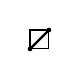
\begin{tikzpicture}[baseline={(0,0)}, scale=0.2]
        \draw (0,0) rectangle (1.2,1.2); % Quadrado
        \draw[thick] (0,0) -- (1.2,1.2); % Diagonal
        \fill (0,0) circle (0.15); % Ponto no início da diagonal
        \fill (1.2,1.2) circle (0.15); % Ponto no fim da diagonal
    \end{tikzpicture}%
}

\newcommand{\retanguloneg}{%
    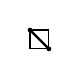
\begin{tikzpicture}[baseline={(0,0)}, scale=0.2]
        \draw (0,0) rectangle (1.2,1.2); % Quadrado
        \draw[thick] (0,1.2) -- (1.2,0); % Diagonal (invertida)
        \fill (0,1.2) circle (0.15); % Ponto no início da diagonal
        \fill (1.2,0) circle (0.15); % Ponto no fim da diagonal
    \end{tikzpicture}%
}

\newcommand{\retangulototal}{%
    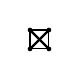
\begin{tikzpicture}[baseline={(0,0)}, scale=0.2]
        \draw (0,0) rectangle (1.2,1.2); % Quadrado
        \draw[thick] (0,1.2) -- (1.2,0); % Diagonal (invertida)
        \draw[thick] (0,0) -- (1.2,1.2); % Diagonal
        \fill (0,1.2) circle (0.15); % Ponto no início da diagonal
        \fill (1.2,0) circle (0.15); % Ponto no fim da diagonal
        \fill (0,0) circle (0.15); % Ponto no início da diagonal
        \fill (1.2,1.2) circle (0.15); % Ponto no fim da diagonal
    \end{tikzpicture}%
}

Neste capítulo entenderemos como a visão geométrica de um algoritmo de busca em ABB para uma sequência de acessos $X$ se relaciona com o custo ótimo $OPT(X)$.

\section{Orientação de retângulos}
%\section{Categoria de retângulos}

Para construção de provas mais sofisticadas, é necessário entender melhor características da geometria dos retângulos formados por pontos de um conjunto. Por conveniência das provas, todas as sequências de acessos desse capítulo possuem tamanho $n$ e todas as chaves são buscadas exatamente uma vez.

Dividiremos os retângulos formados por um par de pontos do conjunto $P$ em dois grupos, os $\retangulopos$-retângulos e os $\retanguloneg$-retângulos. Denotamos por $\retangulopos$\textit{-retângulo} todo retângulo que possuir o vértice à esquerda mais abaixo que o vértice à direita. Denotamos por $\retanguloneg$\textit{-retângulo} todo retângulo que possuir o vértice à esquerda mais abaixo que o vértice à direita.

Assim, definimos que um conjunto de pontos $X$ é $\retangulopos$\textit{-satisfeito} se todos os $\retangulopos$-retângulos formados por dois pontos não ortogonalmente colineares de $X$ são arboreamente satisfeito. Simétrico para a outra orientação.

Também será útil definir quando ambos os tipos de retângulos são satisfeitos. Chamamos um superconjunto $Z$ de $X$ de $\retangulototal$\textit{-satisfeito} se existem subconjuntos $Z_{\retangulopos}$ e $Z_{\retanguloneg}$ de $Z$ tal que $Z_{\retangulopos} \cup X$ é $\retangulopos$-satisfeito e $Z_{\retanguloneg} \cup X$ é $\retanguloneg$-satisfeito.  

%todos os $\retangulopos$-retângulos e os $\retanguloneg$-retângulos são arboreamente satisfeitos, ou seja, $X$ é $\retangulopos$-satisfeito e $\retanguloneg$-satisfeito.

Por fim, definimos \textit{minASS}$_{\retangulopos}(X)$ como o tamanho do menor superconjunto de $X$ que é $\retangulopos$-satisfeito. Analogamente, \textit{minASS}$_{\retanguloneg}(X)$ é o tamanho do menor superconjunto de $X$ que é $\retanguloneg$-satisfeito e \textit{minASS}$_{\retangulototal}(X)$ é o tamanho do menor superconjunto de $X$ que é $\retangulototal$-satisfeito.

\begin{lemma}
    minASS$_{\retangulototal}(X) \leq$ minASS$_{\retangulopos}(X)$ + minASS$_{\retanguloneg}(X)$.
\end{lemma}

\begin{proof}
    
\end{proof}

\begin{lemma}
    minASS$_{\retangulototal}(X) \leq$ minASS$(X)$.
\end{lemma}

\begin{proof}
\end{proof}

\section{Guloso futurista orientado}

Definimos agora dois algoritmos muito parecidos com o guloso futurista visto no capítulo anterior que nos ajudarão a descrever delimitações inferiores em buscas. 

Chamaremos de \textit{futurista}-$\retangulopos$ o algoritmo que dado um conjunto de pontos $P_X$ que representa a sequência $X$ de buscas, inicializa $P = P_X$ e define uma reta horizontal $r$ inicializada em $y = 1$ e indo até $y = m$. Esse algoritmo mantém o invariante que todos os pares de pontos de $P$ em $r$ ou abaixo de $r$ são $\retangulopos$-satisfeitos. Esse algoritmo garante essa propriedade adicionando o menor número de pontos na linha $r$ analisada que garanta essa característica. Ao fim da execução, o conjunto de pontos $P$ é $\retangulopos$-satisfeito.

Chamaremos de $|$\textit{Fut}$_{\retangulopos}(X)|$ o número de pontos adicionados durante a execução do algoritmo guloso futurista $\retangulopos$ para a sequência de acessos $X$. Todas essas definições valem simetricamente para o algoritmo futurista-$\retanguloneg$.
Veja a Figura~\ref{fig:greedy_sign}.

\begin{figure}
    \centering
    \begin{minipage}[b]{0.48\linewidth}
        \centering
        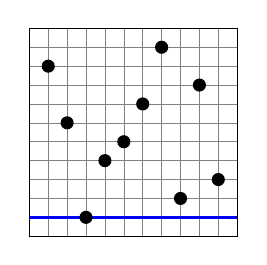
\begin{tikzpicture}[scale=0.24]
            \draw[very thin, gray] (0,0) grid (11,11);
    
            \draw[blue, line width=1.2pt] (0,1) -- (11,1);

            \filldraw[black] (3,1) circle (9pt);
            \filldraw[black] (8,2) circle (9pt);
            \filldraw[black] (10,3) circle (9pt);
            \filldraw[black] (4,4) circle (9pt);
            \filldraw[black] (5,5) circle (9pt);
            \filldraw[black] (2,6) circle (9pt);
            \filldraw[black] (6,7) circle (9pt);
            \filldraw[black] (9,8) circle (9pt);
            \filldraw[black] (1,9) circle (9pt);
            \filldraw[black] (7,10) circle (9pt);
            \draw[black, line width=0.5pt] (0,0) rectangle (11,11); 
        \end{tikzpicture}
        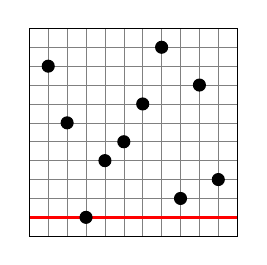
\begin{tikzpicture}[scale=0.24]
            \draw[very thin, gray] (0,0) grid (11,11);
    
            \draw[red, line width=1.2pt] (0,1) -- (11,1);

            \filldraw[black] (3,1) circle (9pt);
            \filldraw[black] (8,2) circle (9pt);
            \filldraw[black] (10,3) circle (9pt);
            \filldraw[black] (4,4) circle (9pt);
            \filldraw[black] (5,5) circle (9pt);
            \filldraw[black] (2,6) circle (9pt);
            \filldraw[black] (6,7) circle (9pt);
            \filldraw[black] (9,8) circle (9pt);
            \filldraw[black] (1,9) circle (9pt);
            \filldraw[black] (7,10) circle (9pt);

            \draw[black, line width=0.5pt] (0,0) rectangle (11,11); 
        \end{tikzpicture}
        \\
        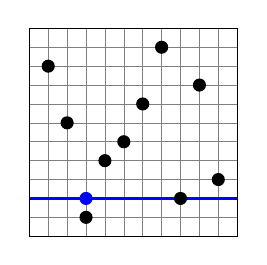
\begin{tikzpicture}[scale=0.24]
            \draw[very thin, gray] (0,0) grid (11,11);
    
            \draw[blue, line width=1.2pt] (0,2) -- (11,2);

            \filldraw[black] (3,1) circle (9pt);
            \filldraw[black] (8,2) circle (9pt);
            \filldraw[black] (10,3) circle (9pt);
            \filldraw[black] (4,4) circle (9pt);
            \filldraw[black] (5,5) circle (9pt);
            \filldraw[black] (2,6) circle (9pt);
            \filldraw[black] (6,7) circle (9pt);
            \filldraw[black] (9,8) circle (9pt);
            \filldraw[black] (1,9) circle (9pt);
            \filldraw[black] (7,10) circle (9pt);

            \filldraw[blue] (3,2) circle (9pt);

            \draw[black, line width=0.5pt] (0,0) rectangle (11,11); 
        \end{tikzpicture}
        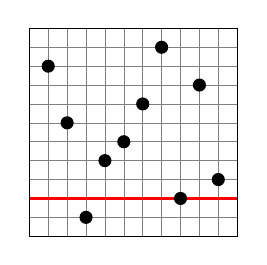
\begin{tikzpicture}[scale=0.24]
            \draw[very thin, gray] (0,0) grid (11,11);
    
            \draw[red, line width=1.2pt] (0,2) -- (11,2);

            \filldraw[black] (3,1) circle (9pt);
            \filldraw[black] (8,2) circle (9pt);
            \filldraw[black] (10,3) circle (9pt);
            \filldraw[black] (4,4) circle (9pt);
            \filldraw[black] (5,5) circle (9pt);
            \filldraw[black] (2,6) circle (9pt);
            \filldraw[black] (6,7) circle (9pt);
            \filldraw[black] (9,8) circle (9pt);
            \filldraw[black] (1,9) circle (9pt);
            \filldraw[black] (7,10) circle (9pt);

            \draw[black, line width=0.5pt] (0,0) rectangle (11,11); 
        \end{tikzpicture}
        \\
        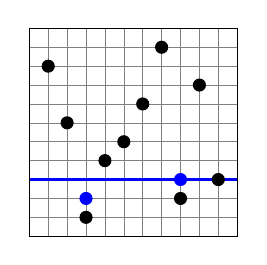
\begin{tikzpicture}[scale=0.24]
            \draw[very thin, gray] (0,0) grid (11,11);
    
            \draw[blue, line width=1.2pt] (0,3) -- (11,3);

            \filldraw[black] (3,1) circle (9pt);
            \filldraw[black] (8,2) circle (9pt);
            \filldraw[black] (10,3) circle (9pt);
            \filldraw[black] (4,4) circle (9pt);
            \filldraw[black] (5,5) circle (9pt);
            \filldraw[black] (2,6) circle (9pt);
            \filldraw[black] (6,7) circle (9pt);
            \filldraw[black] (9,8) circle (9pt);
            \filldraw[black] (1,9) circle (9pt);
            \filldraw[black] (7,10) circle (9pt);

            \filldraw[blue] (3,2) circle (9pt);
            \filldraw[blue] (8,3) circle (9pt);

            \draw[black, line width=0.5pt] (0,0) rectangle (11,11); 
        \end{tikzpicture}
        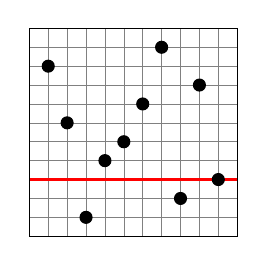
\begin{tikzpicture}[scale=0.24]
            \draw[very thin, gray] (0,0) grid (11,11);
    
            \draw[red, line width=1.2pt] (0,3) -- (11,3);

            \filldraw[black] (3,1) circle (9pt);
            \filldraw[black] (8,2) circle (9pt);
            \filldraw[black] (10,3) circle (9pt);
            \filldraw[black] (4,4) circle (9pt);
            \filldraw[black] (5,5) circle (9pt);
            \filldraw[black] (2,6) circle (9pt);
            \filldraw[black] (6,7) circle (9pt);
            \filldraw[black] (9,8) circle (9pt);
            \filldraw[black] (1,9) circle (9pt);
            \filldraw[black] (7,10) circle (9pt);

            \draw[black, line width=0.5pt] (0,0) rectangle (11,11); 
        \end{tikzpicture}
        \\
        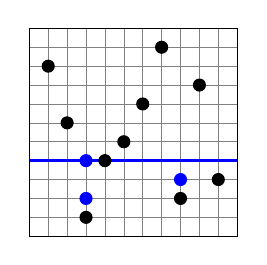
\begin{tikzpicture}[scale=0.24]
            \draw[very thin, gray] (0,0) grid (11,11);
    
            \draw[blue, line width=1.2pt] (0,4) -- (11,4);

            \filldraw[black] (3,1) circle (9pt);
            \filldraw[black] (8,2) circle (9pt);
            \filldraw[black] (10,3) circle (9pt);
            \filldraw[black] (4,4) circle (9pt);
            \filldraw[black] (5,5) circle (9pt);
            \filldraw[black] (2,6) circle (9pt);
            \filldraw[black] (6,7) circle (9pt);
            \filldraw[black] (9,8) circle (9pt);
            \filldraw[black] (1,9) circle (9pt);
            \filldraw[black] (7,10) circle (9pt);


            
            
            \filldraw[blue] (3,2) circle (9pt);
            \filldraw[blue] (8,3) circle (9pt);
            \filldraw[blue] (3,4) circle (9pt);

            \draw[black, line width=0.5pt] (0,0) rectangle (11,11); 
        \end{tikzpicture}
        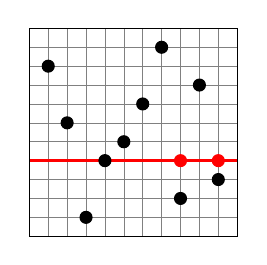
\begin{tikzpicture}[scale=0.24]
            \draw[very thin, gray] (0,0) grid (11,11);
    
            \draw[red, line width=1.2pt] (0,4) -- (11,4);

            \filldraw[black] (3,1) circle (9pt);
            \filldraw[black] (8,2) circle (9pt);
            \filldraw[black] (10,3) circle (9pt);
            \filldraw[black] (4,4) circle (9pt);
            \filldraw[black] (5,5) circle (9pt);
            \filldraw[black] (2,6) circle (9pt);
            \filldraw[black] (6,7) circle (9pt);
            \filldraw[black] (9,8) circle (9pt);
            \filldraw[black] (1,9) circle (9pt);
            \filldraw[black] (7,10) circle (9pt);

            \filldraw[red] (8,4) circle (9pt);
            \filldraw[red] (10,4) circle (9pt);

            \draw[black, line width=0.5pt] (0,0) rectangle (11,11); 
        \end{tikzpicture}
        \\
        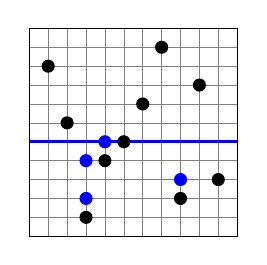
\begin{tikzpicture}[scale=0.24]
            \draw[very thin, gray] (0,0) grid (11,11);
    
            \draw[blue, line width=1.2pt] (0,5) -- (11,5);

            \filldraw[black] (3,1) circle (9pt);
            \filldraw[black] (8,2) circle (9pt);
            \filldraw[black] (10,3) circle (9pt);
            \filldraw[black] (4,4) circle (9pt);
            \filldraw[black] (5,5) circle (9pt);
            \filldraw[black] (2,6) circle (9pt);
            \filldraw[black] (6,7) circle (9pt);
            \filldraw[black] (9,8) circle (9pt);
            \filldraw[black] (1,9) circle (9pt);
            \filldraw[black] (7,10) circle (9pt);
            
            \filldraw[blue] (3,2) circle (9pt);
            \filldraw[blue] (8,3) circle (9pt);
            \filldraw[blue] (3,4) circle (9pt);
            \filldraw[blue] (4,5) circle (9pt);

            \draw[black, line width=0.5pt] (0,0) rectangle (11,11); 
        \end{tikzpicture}
        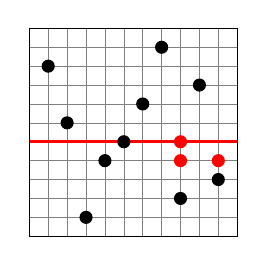
\begin{tikzpicture}[scale=0.24]
            \draw[very thin, gray] (0,0) grid (11,11);
    
            \draw[red, line width=1.2pt] (0,5) -- (11,5);

            \filldraw[black] (3,1) circle (9pt);
            \filldraw[black] (8,2) circle (9pt);
            \filldraw[black] (10,3) circle (9pt);
            \filldraw[black] (4,4) circle (9pt);
            \filldraw[black] (5,5) circle (9pt);
            \filldraw[black] (2,6) circle (9pt);
            \filldraw[black] (6,7) circle (9pt);
            \filldraw[black] (9,8) circle (9pt);
            \filldraw[black] (1,9) circle (9pt);
            \filldraw[black] (7,10) circle (9pt);
            
            \filldraw[red] (8,4) circle (9pt);
            \filldraw[red] (10,4) circle (9pt);
            \filldraw[red] (8,5) circle (9pt);

            \draw[black, line width=0.5pt] (0,0) rectangle (11,11); 
        \end{tikzpicture}
    \end{minipage}
    %\hspace{0.01\linewidth}
    \hfill
    \begin{minipage}[b]{0.48\linewidth}
        \centering
        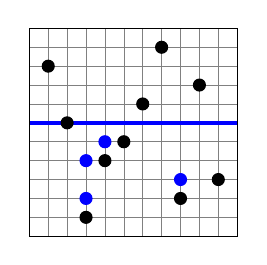
\begin{tikzpicture}[scale=0.24]
            \draw[very thin, gray] (0,0) grid (11,11);
    
            \draw[blue, line width=1.2pt] (0,6) -- (11,6);

            \filldraw[black] (3,1) circle (9pt);
            \filldraw[black] (8,2) circle (9pt);
            \filldraw[black] (10,3) circle (9pt);
            \filldraw[black] (4,4) circle (9pt);
            \filldraw[black] (5,5) circle (9pt);
            \filldraw[black] (2,6) circle (9pt);
            \filldraw[black] (6,7) circle (9pt);
            \filldraw[black] (9,8) circle (9pt);
            \filldraw[black] (1,9) circle (9pt);
            \filldraw[black] (7,10) circle (9pt);
  
            \filldraw[blue] (3,2) circle (9pt);
            \filldraw[blue] (8,3) circle (9pt);
            \filldraw[blue] (3,4) circle (9pt);
            \filldraw[blue] (4,5) circle (9pt);

            \draw[black, line width=0.5pt] (0,0) rectangle (11,11); 
        \end{tikzpicture}
        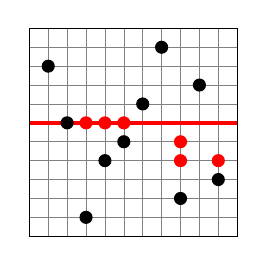
\begin{tikzpicture}[scale=0.24]
            \draw[very thin, gray] (0,0) grid (11,11);
    
            \draw[red, line width=1.2pt] (0,6) -- (11,6);

            \filldraw[black] (3,1) circle (9pt);
            \filldraw[black] (8,2) circle (9pt);
            \filldraw[black] (10,3) circle (9pt);
            \filldraw[black] (4,4) circle (9pt);
            \filldraw[black] (5,5) circle (9pt);
            \filldraw[black] (2,6) circle (9pt);
            \filldraw[black] (6,7) circle (9pt);
            \filldraw[black] (9,8) circle (9pt);
            \filldraw[black] (1,9) circle (9pt);
            \filldraw[black] (7,10) circle (9pt);
            
            \filldraw[red] (8,4) circle (9pt);
            \filldraw[red] (10,4) circle (9pt);
            \filldraw[red] (8,5) circle (9pt);
            \filldraw[red] (3,6) circle (9pt);
            \filldraw[red] (4,6) circle (9pt);
            \filldraw[red] (5,6) circle (9pt);

            \draw[black, line width=0.5pt] (0,0) rectangle (11,11); 
        \end{tikzpicture}
        \\
        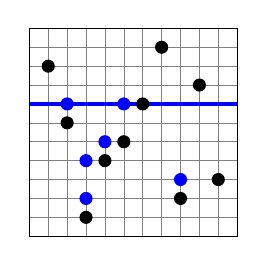
\begin{tikzpicture}[scale=0.24]
            \draw[very thin, gray] (0,0) grid (11,11);
    
            \draw[blue, line width=1.2pt] (0,7) -- (11,7);

            \filldraw[black] (3,1) circle (9pt);
            \filldraw[black] (8,2) circle (9pt);
            \filldraw[black] (10,3) circle (9pt);
            \filldraw[black] (4,4) circle (9pt);
            \filldraw[black] (5,5) circle (9pt);
            \filldraw[black] (2,6) circle (9pt);
            \filldraw[black] (6,7) circle (9pt);
            \filldraw[black] (9,8) circle (9pt);
            \filldraw[black] (1,9) circle (9pt);
            \filldraw[black] (7,10) circle (9pt);
            
            \filldraw[blue] (3,2) circle (9pt);
            \filldraw[blue] (8,3) circle (9pt);
            \filldraw[blue] (3,4) circle (9pt);
            \filldraw[blue] (4,5) circle (9pt);
            \filldraw[blue] (2,7) circle (9pt);
            \filldraw[blue] (5,7) circle (9pt);

            \draw[black, line width=0.5pt] (0,0) rectangle (11,11); 
        \end{tikzpicture}
        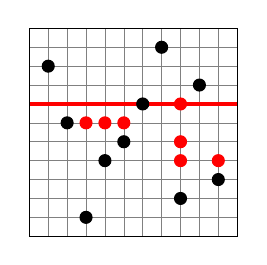
\begin{tikzpicture}[scale=0.24]
            \draw[very thin, gray] (0,0) grid (11,11);
    
            \draw[red, line width=1.2pt] (0,7) -- (11,7);

            \filldraw[black] (3,1) circle (9pt);
            \filldraw[black] (8,2) circle (9pt);
            \filldraw[black] (10,3) circle (9pt);
            \filldraw[black] (4,4) circle (9pt);
            \filldraw[black] (5,5) circle (9pt);
            \filldraw[black] (2,6) circle (9pt);
            \filldraw[black] (6,7) circle (9pt);
            \filldraw[black] (9,8) circle (9pt);
            \filldraw[black] (1,9) circle (9pt);
            \filldraw[black] (7,10) circle (9pt);
            
            \filldraw[red] (8,4) circle (9pt);
            \filldraw[red] (10,4) circle (9pt);
            \filldraw[red] (8,5) circle (9pt);
            \filldraw[red] (3,6) circle (9pt);
            \filldraw[red] (4,6) circle (9pt);
            \filldraw[red] (5,6) circle (9pt);
            \filldraw[red] (8,7) circle (9pt);

            \draw[black, line width=0.5pt] (0,0) rectangle (11,11); 
        \end{tikzpicture}   
        \\
        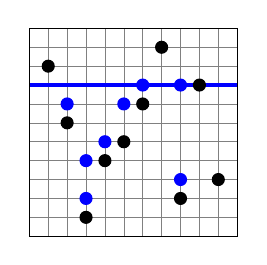
\begin{tikzpicture}[scale=0.24]
            \draw[very thin, gray] (0,0) grid (11,11);
    
            \draw[blue, line width=1.2pt] (0,8) -- (11,8);

            \filldraw[black] (3,1) circle (9pt);
            \filldraw[black] (8,2) circle (9pt);
            \filldraw[black] (10,3) circle (9pt);
            \filldraw[black] (4,4) circle (9pt);
            \filldraw[black] (5,5) circle (9pt);
            \filldraw[black] (2,6) circle (9pt);
            \filldraw[black] (6,7) circle (9pt);
            \filldraw[black] (9,8) circle (9pt);
            \filldraw[black] (1,9) circle (9pt);
            \filldraw[black] (7,10) circle (9pt);            
            
            \filldraw[blue] (3,2) circle (9pt);
            \filldraw[blue] (8,3) circle (9pt);
            \filldraw[blue] (3,4) circle (9pt);
            \filldraw[blue] (4,5) circle (9pt);
            \filldraw[blue] (2,7) circle (9pt);
            \filldraw[blue] (5,7) circle (9pt);
            \filldraw[blue] (6,8) circle (9pt);
            \filldraw[blue] (8,8) circle (9pt);

            \draw[black, line width=0.5pt] (0,0) rectangle (11,11); 
        \end{tikzpicture}
        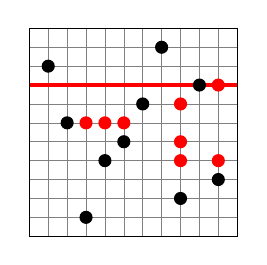
\begin{tikzpicture}[scale=0.24]
            \draw[very thin, gray] (0,0) grid (11,11);
    
            \draw[red, line width=1.2pt] (0,8) -- (11,8);

            \filldraw[black] (3,1) circle (9pt);
            \filldraw[black] (8,2) circle (9pt);
            \filldraw[black] (10,3) circle (9pt);
            \filldraw[black] (4,4) circle (9pt);
            \filldraw[black] (5,5) circle (9pt);
            \filldraw[black] (2,6) circle (9pt);
            \filldraw[black] (6,7) circle (9pt);
            \filldraw[black] (9,8) circle (9pt);
            \filldraw[black] (1,9) circle (9pt);
            \filldraw[black] (7,10) circle (9pt);

            \filldraw[red] (8,4) circle (9pt);
            \filldraw[red] (10,4) circle (9pt);
            \filldraw[red] (8,5) circle (9pt);
            \filldraw[red] (3,6) circle (9pt);
            \filldraw[red] (4,6) circle (9pt);
            \filldraw[red] (5,6) circle (9pt);
            \filldraw[red] (8,7) circle (9pt);
            \filldraw[red] (10,8) circle (9pt);

            \draw[black, line width=0.5pt] (0,0) rectangle (11,11); 
        \end{tikzpicture}
        \\
        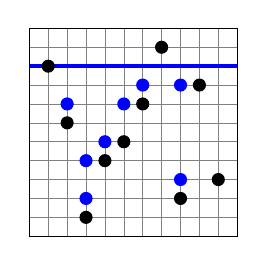
\begin{tikzpicture}[scale=0.24]
            \draw[very thin, gray] (0,0) grid (11,11);
    
            \draw[blue, line width=1.2pt] (0,9) -- (11,9);

            \filldraw[black] (3,1) circle (9pt);
            \filldraw[black] (8,2) circle (9pt);
            \filldraw[black] (10,3) circle (9pt);
            \filldraw[black] (4,4) circle (9pt);
            \filldraw[black] (5,5) circle (9pt);
            \filldraw[black] (2,6) circle (9pt);
            \filldraw[black] (6,7) circle (9pt);
            \filldraw[black] (9,8) circle (9pt);
            \filldraw[black] (1,9) circle (9pt);
            \filldraw[black] (7,10) circle (9pt);
            
            \filldraw[blue] (3,2) circle (9pt);
            \filldraw[blue] (8,3) circle (9pt);
            \filldraw[blue] (3,4) circle (9pt);
            \filldraw[blue] (4,5) circle (9pt);
            \filldraw[blue] (2,7) circle (9pt);
            \filldraw[blue] (5,7) circle (9pt);
            \filldraw[blue] (6,8) circle (9pt);
            \filldraw[blue] (8,8) circle (9pt);

            \draw[black, line width=0.5pt] (0,0) rectangle (11,11); 
        \end{tikzpicture}
        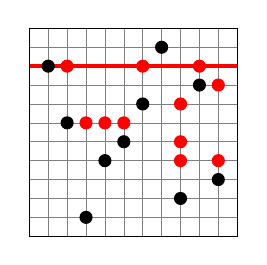
\begin{tikzpicture}[scale=0.24]
            \draw[very thin, gray] (0,0) grid (11,11);
    
            \draw[red, line width=1.2pt] (0,9) -- (11,9);

            \filldraw[black] (3,1) circle (9pt);
            \filldraw[black] (8,2) circle (9pt);
            \filldraw[black] (10,3) circle (9pt);
            \filldraw[black] (4,4) circle (9pt);
            \filldraw[black] (5,5) circle (9pt);
            \filldraw[black] (2,6) circle (9pt);
            \filldraw[black] (6,7) circle (9pt);
            \filldraw[black] (9,8) circle (9pt);
            \filldraw[black] (1,9) circle (9pt);
            \filldraw[black] (7,10) circle (9pt);

            \filldraw[red] (8,4) circle (9pt);
            \filldraw[red] (10,4) circle (9pt);
            \filldraw[red] (8,5) circle (9pt);
            \filldraw[red] (3,6) circle (9pt);
            \filldraw[red] (4,6) circle (9pt);
            \filldraw[red] (5,6) circle (9pt);
            \filldraw[red] (8,7) circle (9pt);
            \filldraw[red] (10,8) circle (9pt);
            \filldraw[red] (2,9) circle (9pt);
            \filldraw[red] (6,9) circle (9pt);
            \filldraw[red] (9,9) circle (9pt);

            \draw[black, line width=0.5pt] (0,0) rectangle (11,11); 
        \end{tikzpicture}
        \\
        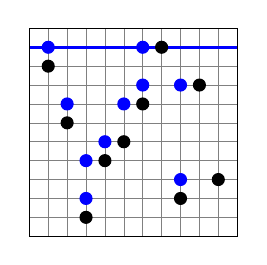
\begin{tikzpicture}[scale=0.24]
            \draw[very thin, gray] (0,0) grid (11,11);
    
            \draw[blue, line width=1.2pt] (0,10) -- (11,10);

            \filldraw[black] (3,1) circle (9pt);
            \filldraw[black] (8,2) circle (9pt);
            \filldraw[black] (10,3) circle (9pt);
            \filldraw[black] (4,4) circle (9pt);
            \filldraw[black] (5,5) circle (9pt);
            \filldraw[black] (2,6) circle (9pt);
            \filldraw[black] (6,7) circle (9pt);
            \filldraw[black] (9,8) circle (9pt);
            \filldraw[black] (1,9) circle (9pt);
            \filldraw[black] (7,10) circle (9pt);
            
            \filldraw[blue] (3,2) circle (9pt);
            \filldraw[blue] (8,3) circle (9pt);
            \filldraw[blue] (3,4) circle (9pt);
            \filldraw[blue] (4,5) circle (9pt);
            \filldraw[blue] (2,7) circle (9pt);
            \filldraw[blue] (5,7) circle (9pt);
            \filldraw[blue] (6,8) circle (9pt);
            \filldraw[blue] (8,8) circle (9pt);
            \filldraw[blue] (1,10) circle (9pt);
            \filldraw[blue] (6,10) circle (9pt);

            \draw[black, line width=0.5pt] (0,0) rectangle (11,11); 
        \end{tikzpicture}
        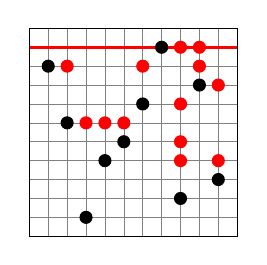
\begin{tikzpicture}[scale=0.24]
            \draw[very thin, gray] (0,0) grid (11,11);
    
            \draw[red, line width=1.2pt] (0,10) -- (11,10);

            \filldraw[black] (3,1) circle (9pt);
            \filldraw[black] (8,2) circle (9pt);
            \filldraw[black] (10,3) circle (9pt);
            \filldraw[black] (4,4) circle (9pt);
            \filldraw[black] (5,5) circle (9pt);
            \filldraw[black] (2,6) circle (9pt);
            \filldraw[black] (6,7) circle (9pt);
            \filldraw[black] (9,8) circle (9pt);
            \filldraw[black] (1,9) circle (9pt);
            \filldraw[black] (7,10) circle (9pt);
            
            \filldraw[red] (8,4) circle (9pt);
            \filldraw[red] (10,4) circle (9pt);
            \filldraw[red] (8,5) circle (9pt);
            \filldraw[red] (3,6) circle (9pt);
            \filldraw[red] (4,6) circle (9pt);
            \filldraw[red] (5,6) circle (9pt);
            \filldraw[red] (8,7) circle (9pt);
            \filldraw[red] (10,8) circle (9pt);
            \filldraw[red] (2,9) circle (9pt);
            \filldraw[red] (6,9) circle (9pt);
            \filldraw[red] (9,9) circle (9pt);
            \filldraw[red] (8,10) circle (9pt);
            \filldraw[red] (9,10) circle (9pt);

            \draw[black, line width=0.5pt] (0,0) rectangle (11,11); 
        \end{tikzpicture}
    \end{minipage}
    \caption{Em preto, $P_X$ da sequência $X = (3,8,10,4,5,2,6,9,1,7)$ de acessos. Em azul, o \protect\retangulopos-futurista para $P_X$ e em vermelho, o \protect\retanguloneg-futurista.}
\label{fig:greedy_sign}
\end{figure}

\section{Independência de retângulos}

Sejam $a$, $b$, $c$ e $d$ pontos de um conjunto $P$.
Denotamos o par $\{a,b\}$-retângulo e $\{c,d\}$-retângulo por \textit{retângulos independentes} se ambos os retângulos são arboreamente insatisfeitos e não há nenhum vértice de algum dos retângulos estritamente no interior do outro. Veja a Figura~\ref{fig:retangulos_independentes}.

\begin{figure}
    \hspace{0.05cm}
    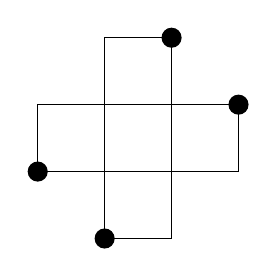
\begin{tikzpicture}[scale=0.85]
        \draw (1,1) rectangle (4,2); % Quadrado
        \draw (2,0) rectangle (3,3); % Quadrado
        \fill (2,0) circle (0.15);
        \fill (1,1) circle (0.15);
        \fill (3,3) circle (0.15);
        \fill (4,2) circle (0.15);
    \end{tikzpicture}
    \hspace{0.2cm}
    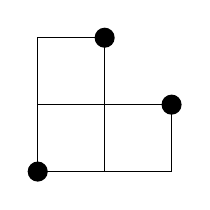
\begin{tikzpicture}[scale=0.85]
        \draw (0,0) rectangle (1,2); % Quadrado
        \draw (0,0) rectangle (2,1); % Quadrado
        \fill (0,0) circle (0.15);
        \fill (1,2) circle (0.15);
        \fill (2,1) circle (0.15);
    \end{tikzpicture}
    \hspace{0.2cm}
    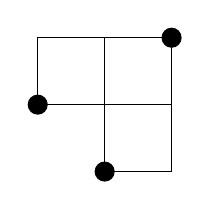
\begin{tikzpicture}[scale=0.85]
        \draw (0,1) rectangle (2,2); % Quadrado
        \draw (1,0) rectangle (2,2); % Quadrado
        \fill (0,1) circle (0.15);
        \fill (1,0) circle (0.15);
        \fill (2,2) circle (0.15);
    \end{tikzpicture}
    \hspace{0.5cm}
    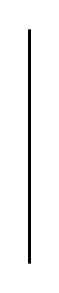
\begin{tikzpicture}[scale=0.85]
        \draw[very thick] (0,-0.5) rectangle (0,3);
    \end{tikzpicture}
    \hspace{0.5cm}
    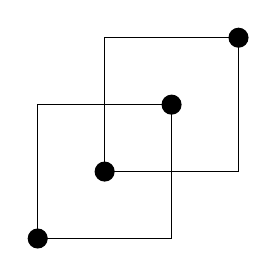
\begin{tikzpicture}[scale=0.85]
        \draw (0,0) rectangle (2,2); % Quadrado
        \draw (1,1) rectangle (3,3); % Quadrado
        \fill (0,0) circle (0.15);
        \fill (1,1) circle (0.15);
        \fill (2,2) circle (0.15);
        \fill (3,3) circle (0.15);
    \end{tikzpicture}
    \hspace{0.2cm}
    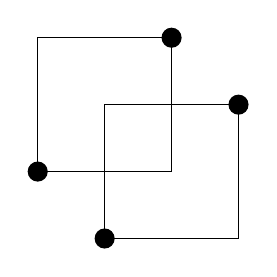
\begin{tikzpicture}[scale=0.85]
        \draw (0,1) rectangle (2,3); % Quadrado
        \draw (1,0) rectangle (3,2); % Quadrado
        \fill (0,1) circle (0.15);
        \fill (1,0) circle (0.15);
        \fill (3,2) circle (0.15);
        \fill (2,3) circle (0.15);
    \end{tikzpicture}
    \caption{Todas as combinações de \protect\retangulopos-retângulos que possuem alguma área no interior em comum. À esquerda, os retângulos independentes e à direita, os retângulos dependentes.}
\label{fig:retangulos_independentes}
\end{figure}


\begin{figure}
    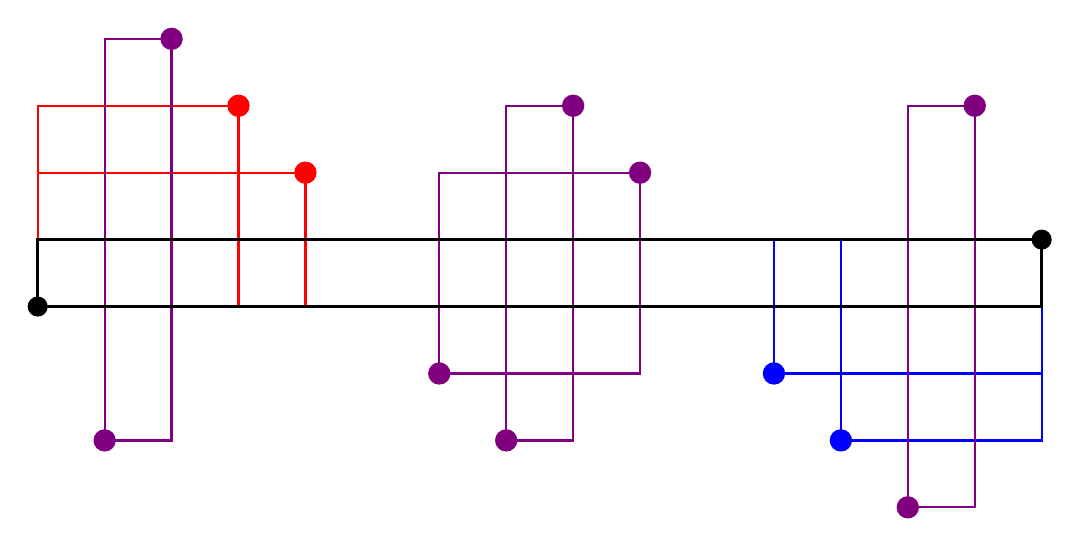
\begin{tikzpicture}[scale=0.85]
        \draw[draw=red, thick] (0,1) rectangle (4,3);
        \draw[draw=red, thick] (0,1) rectangle (3,4);
        \draw[draw=violet, thick] (1,-1) rectangle (2,5);
        
        \fill (0,1) circle (0.15);
        \fill (15,2) circle (0.15);
        \fill[draw=red, fill=red, thick] (4,3) circle (0.15);
        \fill[draw=red, fill=red, thick] (3,4) circle (0.15);
        \fill[draw=violet, fill=violet, thick] (1,-1) circle (0.15);
        \fill[draw=violet, fill=violet, thick] (2,5) circle (0.15);
        
        
        \draw[draw=violet, thick] (6,0) rectangle (9,3);
        \draw[draw=violet, thick] (7,-1) rectangle (8,4);
        \fill[draw=violet, fill=violet, thick] (6,0) circle (0.15);
        \fill[draw=violet, fill=violet, thick] (9,3) circle (0.15);
        \fill[draw=violet, fill=violet, thick] (7,-1) circle (0.15);
        \fill[draw=violet, fill=violet, thick] (8,4) circle (0.15);
        
        
        \draw[draw=blue, thick] (15,2) rectangle (11,0);
        \draw[draw=blue, thick] (15,2) rectangle (12,-1);
        \draw[draw=violet, thick] (14,-2) rectangle (13,4);
        \fill[draw=blue, fill=blue, thick] (12,-1) circle (0.15);
        \fill[draw=blue, fill=blue, thick] (11,0) circle (0.15);
        
        \fill[draw=violet, fill=violet, thick] (13,-2) circle (0.15);
        \fill[draw=violet, fill=violet, thick] (14,4) circle (0.15);
        \draw[very thick] (0,1) rectangle (15,2);
    \end{tikzpicture}
    \caption{Em preto, o $\{a,b\}$-retângulo sendo analisado. Em vermelho, os retângulos independentes que compartilham o vértice $a$. Em azul, os retângulos independentes que compartilham o vértice $b$. Em roxo, os retângulos independentes que não compartilham vértice em comum com o $\{a,b\}$-retângulo.   }
\end{figure}

\begin{lemma}
    Para toda sequência de acessos $X$, existe um conjunto de $\retangulopos$-retângulos independentes IRB$_{\retangulopos}$$(X)$ tal que $|$IRB$_{\retangulopos}(X)| = |$Fut$_{\retangulopos}(X)|$.
\end{lemma}

\begin{lemma}
    Dado um conjunto $Y$ de pontos $\retangulopos$-satisfeito com coordenadas $x$ inteiras, dois pontos $a$ e $b$ não ortogonalmente colineares tal que $a,b \in Y$ e uma linha vertical $l$ com coordenada $x$ não inteira estritamente entre $a.x$ e $b.x$. Então, é possível encontrarmos dois pontos $p,q \in Y$ tal que $p.y = q.y$, $p$ está a esquerda de $l$ e $q$ está a direita de $l$ e não há nenhum ponto de $Y$ no segmento de reta horizontal que conecta $p$ e $q$. 
\end{lemma}

\begin{lemma}
    Dado um conjunto $I$ de retângulos independentes em um conjunto de pontos $X$ tal que todo ponto tem coordenada $x$ distinta e inteira, existe um $\{a,b\}$-retângulo $\in I$ e uma reta vertical $l$ em uma coordenada $x$ não inteira estritamente entre $a.x$ e $b.x$ tal que dentro deste $\{a,b\}$-retângulo $l$ não intersecta o interior de nenhum retângulo de $I \setminus \{\{a,b\}$-retângulo$\}$.
\end{lemma}

\begin{lemma}
    Dado um conjunto $I$ de $\retangulopos$-retângulos independentes em um conjunto de pontos $X$, qualquer superconjunto $Y$ de $X$ que seja $\retangulopos$-satisfeito tem pelos cardinalidade $|I| + |X|$. 
\end{lemma}

\begin{lemma}
    Para qualquer conjunto de pontos $X$, minASS$_{\retangulopos}(X) = |$Fut$_{\retangulopos}(X)| + |X|$.
\end{lemma}

\begin{theorem}
    Se um conjunto de pontos $X$ contém um conjunto $I$ de retângulos independentes, então minASS$_{\retangulopos}(X)$.
\end{theorem}